\documentclass[conference]{IEEEtran}
\ifCLASSINFOpdf

\newcommand{\redcolor}[1]{\textcolor{red}{#1}}

\newcommand{\figref}[1]{Figure~\ref{#1}}
\newcommand{\secref}[1]{Section~\ref{#1}}
\newcommand{\tabref}[1]{Table~\ref{#1}}
\newcommand{\algoref}[1]{Algorithm~\ref{#1}}
\usepackage{graphicx}
\usepackage{subfig}
\usepackage{blindtext}
\usepackage{array}
\usepackage{caption}
\usepackage{url}
\usepackage{epstopdf}
\usepackage{multirow}
\usepackage{xcolor,colortbl}

\newcommand{\pushline}{\Indp}
\definecolor{Gray}{gray}{0.91}
\newcolumntype{a}{>{\columncolor{Gray}}c}

\newcommand{\indic}{INDiC }
\newcommand{\indicns}{INDiC }

\else
\fi

\usepackage[boxed,ruled,vlined]{algorithm2e}

% *** ALIGNMENT PACKAGES ***
\hyphenation{op-tical net-works semi-conduc-tor}


\begin{document}
%
% paper title
% can use linebreaks \\ within to get better formatting as desired
\title{INDiC: Improved Non intrusive load monitoring using load Division and Calibration}


\author{\IEEEauthorblockN{Nipun Batra}
\IEEEauthorblockA{Indraprastha Institute of Information Technology\\
India\\
}
\and
\IEEEauthorblockN{Author2}
\IEEEauthorblockA{Twentieth Century Fox\\
Springfield, USA\\
Email: homer@thesimpsons.com}
\and
\IEEEauthorblockN{James Kirk}
\IEEEauthorblockA{Starfleet Academy\\
San Francisco, California 96678-2391\\
Fax: (888) 555--1212}}
% make the title area
\maketitle


\begin{abstract}
%\boldmath
Buildings Non-Intrusive appliance load monitoring (NIALM) is the process of disaggregating the overall electricity usage into constituent appliances. In this paper we extend the Combinatorial Optimization (CO) approach for disaggregation, which was originally proposed in the seminal work on NIALM, in following two ways: 1) Breaking the problem into subproblems and reducing the state space; 2) Applying additional constraints backed by sound domain expertise. We evaluate our approach using REDD dataset and show practical problems which need to be solved while dealing with the dataset. We also propose a metric for evaluating NILM, which we believe overcomes many shortcomings of commonly used metrics.
\end{abstract}
\IEEEpeerreviewmaketitle



\section{Introduction}
\noindent Buildings account for significant proportion of overall energy use in both the developing (e.g. 47\% of total energy in India~\cite{evans09}) and the developed (e.g. 41\% and 45\% in US and UK respectively) countries. Modest improvements in building energy use can result in significant aggregate impact at the national scale. While several automation and management systems have been proposed for improving the operational efficiency of building systems, such systems typically lack the ability to provide detailed consumption information (e.g. appliance level consumption). Prior work~\cite{darby} has shown that better feedback systems, enabling appliance level consumption, that provide insights about occupant's energy usage information further encourages energy saving behavior resulting in 5-15\% savings in electricity usage.

\noindent Measuring each appliance's consumption separately, for providing such a feedback, is both prohibitively expensive and difficult to manage. Alternatively, prior research has proposed Non Intrusive Appliance Load Monitoring (NIALM) that involves separating the aggregated electricity consumption obtained at the meter level into individual appliance consumption. Several modeling and inference approaches have been proposed (e.g. Factorial Hidden Markov Model~\cite{Ghahramani_97a}, Combinatorial Optimization~\cite{hart}) in the past to address NIALM with varied level of accuracy. NIALM work typically assumes that all the loads are assigned to the same meter. However, many practical scenarios (e.g. use of 2-phase supply in many homes in USA and 3-phase supply for many homes in India) involve load division across different phases coming at the home level. Automated assignment of different loads in a home to each phase followed by NIALM application on each phase separately can reduce the overall modeling and inference complexity. 

\noindent Further, the measurements, both at the meter level and at the appliance level, are often taken with different equipments (Current Transformers, in-line measurements, ICs\footnote{Example IC for power measurement is Maxim 78M6612}) each with their own accuracy levels. Calibrating these diverse measurements will be beneficial for NIALM modeling and inference. Grid conditions such as voltage fluctuations further motivate calibration. Motivated by these practical scenarios, we propose \indic - \textbf{I}mproved \textbf{N}IALM using load \textbf{Di}vision and \textbf{C}alibration. Specific research condtributions of our work are:
\begin{itemize}
\item Novel approach named \indic that involves two simple pre-processing steps - Load Division (i.e. automated assignment of different loads in a home to each of the separate Mains) and Calibration (accounting for varied measurement accuracy across different equipments), that can be applied in a generic manner across several proposed NIALM modeling and inference approaches to further improve their accuracy. 
\item Extensive empirical validation, using publicly available REDD~\cite{redd} dataset, establishing the effectiveness of \indicns, specifically for Combinatorial Optimization based NIALM. 
\item Release of open source implementation of the proposed work\footnote{Add link to website} for comparative analysis with other NIALM approaches as an IPython notebook\footnote{\url{http://www.ipython.org}}. 
\end{itemize}
\noindent We believe that this is the first extensive release of a generic NIALM code base that can be used across many of the publicly available datasets and with several existing NIALM modeling and inference approaches.


\section{Related work}
\noindent Non-intrusive appliance load monitoring was first studied by Hart~\cite{hart} in the early 1990s by examining signatures in aggregated load to indicate activities of appliances. The problem has been well studied in recent years (\cite{survey1,survey2,survey3}) and NIALM systems can broadly be divided into two categories based on whether supervised or unsupervised disaggregation methods are used.
%\begin{itemize}
%\item \textbf{Frequency of data collection}:[REWRITE] Approaches such as harmonic analysis require data to be sampled at more than a thousand samples a second. Whereas approaches 
%\textbf{Supervised/Unsupervised}: 
\noindent Supervised learning techniques include optimization-based methods such as integer programming \cite{Suzuki_08} and genetic algorithms \cite{Baranski_04}. These approaches are compute intensive and appliances with similar or overlapping load signatures are difficult to discern. Other machine learning techniques (such as Artificial Neural Network (ANNs) \cite{Ruzzelli_10} and Hidden Markov Models (HMM) \cite{Zia_11}), have also been shown to work well for the task. Variants of HMMs such as factorial hidden Markov models (FHMMs) \cite{Ghahramani_97a}, additive FHMMs \cite{Kolter_12}, conditional factorial hidden semi-Markov models \cite{Kim_11} and difference HMMs \cite{parson2012_aaai} have been studied. In factorial HMMs several models evolve independently and in parallel and the observed output is some joint function of all the hidden states; additive HMMs allow emission of a single real-valued (unobserved) output from each HMM and the output is the sum of these HMMs. In difference HMMs \cite{parson2012_aaai} each appliance's load is modeled using a graphical model and it is disaggregated from the aggregate power -- this process is repeated iteratively until all appliances for which general models are available are disaggregated. It is therefore possible to infer the probability that a change in aggregated power was generated by two consecutive states of an appliance. The applicability of these sophisticated techniques are generally hindered by the difficulty of inference from models with a large number of HMMs. Rahayu et. al. \cite{Rahayu_12} propose a discriminative model for energy disaggregation that predicts the most likely appliance state configuration from aggregated load using nonparametric classification algorithms. They posit that ``subset sum" type techniques are not very effective since a large portion of the home energy is not monitored directly. In this paper, we put forward a simple idea -- the aggregated load can be further split up by information on mains and knowing which appliance is assigned to which main. This would make the task of disaggregation inherently easier by solving a simpler optimization problem and most of the above sophisticated machine learning based modeling approaches can still be applied to the task\footnote{The use of combinatorial optimization is only for the purpose of illustration and there is clearly no requirement to adhere to this modeling technique alone.}. 

%\end{itemize}
\noindent Several datasets have been made publicly available for benchmarking energy disaggregation algorithms including REDD\cite{redd}, Blued\cite{blued_cmu}, Pecan\cite{pecan} and Smart*\cite{smart}. Our empirical analysis is on the REDD data primarily because this is the most popular data set for evaluating state-of-the-art NIALM approaches. 
%When you do the comparison, bring up how is your work different rather than just saying X did A and Y did B.
%\begin{itemize}
%\item Classification of different NIALM approaches - High/Low frequency, Time/Frequency domain analysis, supervised/unsupervised~\cite{survey1,survey2,survey3}.

%For a more detailed overview the reader is referred to the above mentioned survey papers.

%%\item Discuss the modeling approaches that are used
%%\begin{itemize}
%%\item Additive Factorial HMM
%%\item Difference HMM \cite{parson2012_aaai}
%%\end{itemize}

%\item Datasets used: Recent datasets have spurred this field
%\begin{itemize}
%\item REDD \cite{redd}
%\item Blued \cite{blued_cmu}
%\item Smart* \cite{smart}
%\end{itemize}

%\end{itemize}
\section{NIALM}
%\noindent NIALM is the process of disaggregating the total electrical load into constituent appliances \cite{hart}.
\noindent A typical NIALM setup involves measuring the power mains with smart meters and individual appliances with appliance meters for ground truth. The NIALM problem in supervised setting is formulated as predicting the power sequence for $n^{th}$ appliance, $y^n$, given the measured power sequence for each appliance $\theta^n$ (measured via appliance meters) and the total aggregate power sequence $x$ (measured via smart meters). Remaining terminologies and functions are defined in \tabref{tab:terms} \cite{redd,parson2012_aaai,hart}. \figref{fig:disagg} shows the process of disaggregation applied to a house mains, whereby the consumption patterns of 3 appliances: refrigerator, lighting and microwave can be seen. It must be highlighted that it is improbable to instrument all the appliances in a home, thus, there will be some unaccounted power, which can also be seen in the figure. We now explain Combinatorial optimization which was proposed by Hart \cite{hart} for solving NIALM.

\begin{figure} 
	
    \subfloat[\scriptsize Aggregate home power measured by smart meter]{
    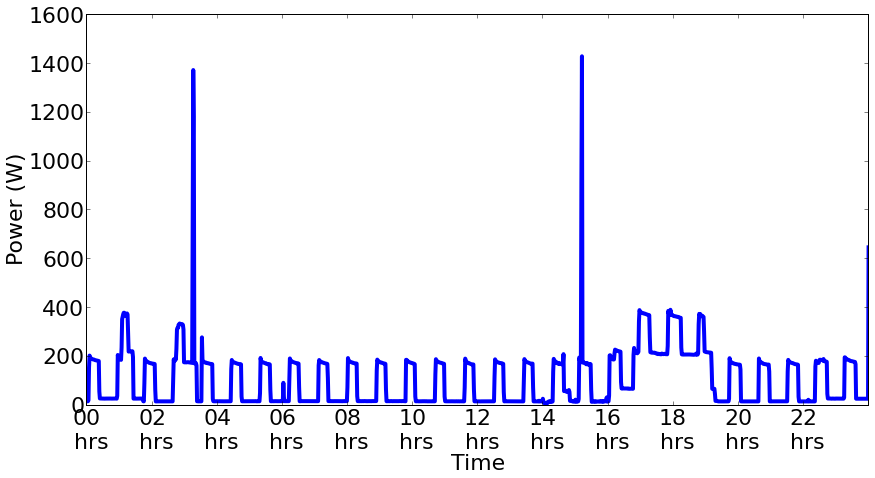
\includegraphics[scale=0.145]{./figures/before_disagg_2.png}}
%    \hspace{0.2pt}
    \subfloat[\scriptsize Aggregate home power disaggregated into 3 appliances: refrigerator, lighting and microwave. Some power is unaccounted as complete information about all appliances is not available. ]{
        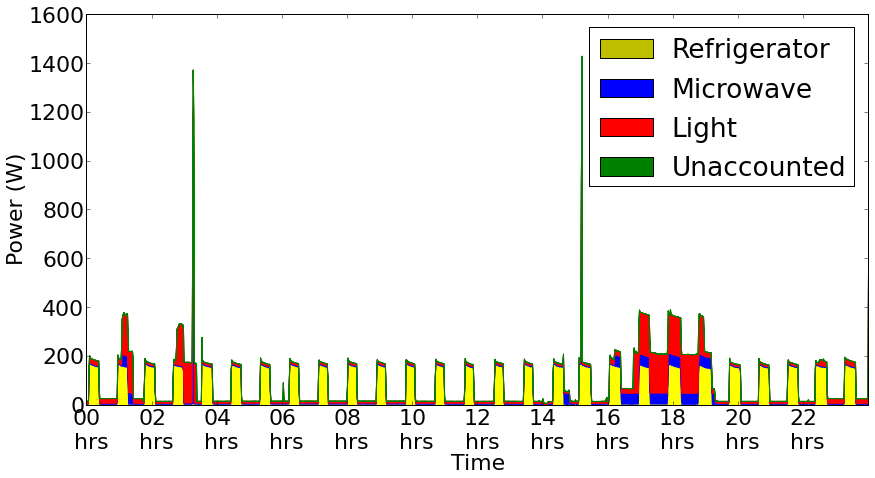
\includegraphics[scale=0.145]{./figures/after_disagg_2.png}}
     \vspace{-8pt}
  	\caption{Disaggregating a home's electrical mains}
    \label{fig:disagg}
    \vspace{-8pt}
\end{figure}
%\noindent We use some terminologies from previous work  and extend them for our analysis in \tabref{tab:terms}. Based on these terminologies, 


\begin{table}[ht!]
\vspace{-12pt}
\caption{Terminologies and Functions}
\vspace{-10pt}
\label{tab:terms}
\begin{tabular}{|l|l|}
\hline
Symbol&Meaning\\[0.1cm]
\hline
$t\in {1,..T}$& Time slice\\[0.1cm]
\hline
$n\in{1,..N}$ & Appliance number\\[0.1cm]
\hline
$\theta^n=\{\theta_1^n,...,\theta_T^n\}$ & Measured power sequence for $n^{th}$ appliance\\[0.1cm]
\hline
$\theta^{M_1}=\{\theta_1^{M_1},...,\theta_T^{M_1}\}$ & Measured power sequence for Mains 1\\[0.1cm]
\hline
$\theta^{M_2}=\{\theta_1^{M_2},...,\theta_T^{M_2}\}$ & Measured power sequence for Mains 2\\[0.1cm]
\hline
$x=\{ x_1,..,x_T\}=$ & Measured aggregate power sequence\\[0.1cm]
$\theta^{M_1}+\theta^{M_2}$ &\\[0.1cm]
\hline
%$v=\{ v_1,..,v_T\}$ & Labeled voltage time series\\[0.1cm]
%$e^{M_1}=\{e_1^{M_1},...,e_T^{M_1}\}$ & Noise power sequence for Mains 1\\[0.1cm]
%$e^{M_2}=\{e_1^{M_2},...,e_T^{M_2}\}$ & Noise power sequence for Mains 2\\[0.1cm]
$e=\{e_1,...,e_T\}$ & Aggregate noise power sequence\\[0.1cm]
\hline
$p$ & Number of electrical mains in a home\\[0.1cm]
\hline
$N_i \:where\:i \in {1,p}$ & Number of loads in $i^{th}$ mains\\[0.1cm]
\hline
$y^n=\{y_1^n,..y_T^n\}$ & Predicted power sequence for $n^{th}$ appliance\\[0.1cm]
\hline
$k\in {1,..K}$ & Appliance power state\\[0.1cm]
\hline
$z^n=\{z_1^n,..z_T^n\}$ & Appliance state sequence for $n^{th}$ \\[0.1cm]
& appliance,$z_i^n \in [1,..K]$\\[0.1cm]
\hline
$z_{t,k}^n \in{0,1}$ & Whether $n^{th}$ appliance is in $k^{th}$ state at time $t$\\[0.1cm]
\hline 
$\mu^n=\{\mu_1^n,..\mu_K^n\}$ & Power draw by $n^{th}$ appliance in $k^{th}$ state\\[0.1cm]
\hline
$\theta^n_{k^1,k^2}$& Measured power sequence when $n^{th}$ appliance \\[0.1cm]
& transitions from $k^1$ to $k^2$ state\\[0.1cm]
\hline
$Mapping[n] \in {M_i}$ & Mapping of $n^{th}$ appliance to $i^{th}$ Mains\\[0.1cm]
where $i \in {1,2}$ & \\
\hline 
$s_t$ & Value of a timeseries $s$ at time $t$ \\
\hline
$Event(s,threshold)$ & An event in timeseries $s$ occurs \\
&when $|s_t-s_{t-1}|>threshold$\\
& An event has an associated $time$ $t$\\
& and $magnitude$ $|s_t-s_{t-1}|$\\
%\hline
%\multirow{2}{*}{$B$} & List of background appliances (which can run\\[0.1cm]
% 					 &without human intervention) eg. refrigerator\\[0.1cm]
%\multirow{2}{*}{$F$} & List of foreground appliances (which are \\[0.1cm] 
% 					 &operated by humans) eg. light, microwave\\[0.1cm]
\hline
\hline
$Downsample(s,filter,$ & Function to downsample a timeseries $s$ to\\[0.1cm]
$resolution)$                                        & a $resolution$ according to specified $filter$\\[0.1cm]
%$Normalize(s,v,$ & Function to normalize a power timeseries $s$\\[0.1cm]
%$Rated\_Voltage)$                                 & given voltage timeseries $v$ according to\\[0.1cm]
%                                    &the formula: $(\frac{Rated\_Voltage}{v})^2s$\\[0.1cm]
\hline
$Timeseries\_sync([s^1,..s^n]$ & Function to ensure that $n$ timeseries start and\\[0.1cm]
$,method)$                                        &end at same times and handling missing\\[0.1cm]
                                        & data using specified $method$\\[0.1cm]
\hline                                        
$Sort([s^1,..s^n],$ & Function to sort $n$ timeseries according\\[0.1cm]
$parameter,order)$  &to $parameter$ in specified $order$\\[0.1cm]
%$Contiguous\_Below\_$ & Function to find contiguous period where time \\[0.1cm]
%$Mean(s,min\_period)$                  &series $s$ is below its mean \\[0.1cm]
%                                       &for atleast $min\_period$\\[0.1cm]
\hline
$Event\_Detection(s,$ & Function returning magnitude and times of \\[0.1cm]
$threshold)$                  &$Events(s,threshold)$ in timeseries $s$\\[0.1cm]

                             
%\multirow{2}{*}{$Greater\_Than(s,threshold)$} & Function to return times when timeseries $s$ is\\[0.1cm]
%                                        &greater than $threshold$\\[0.1cm]                                                                                                    
                                                                               

\hline
%
\end{tabular}
\end{table}

\noindent \textbf{Combinatorial Optimization(CO)}: At a given time an appliance can only be in a single state which is given by:

$\sum\limits_{k=1}^{k=K} z_{t,k}^n=1$ 

\noindent The power consumption by $n^{th}$ appliance in $k^{th}$ state at time $t$ is given by:

$\hat{\theta}^n_{t,k}=\sum\limits_{k=1}^{K} z_{t,k}^n \mu_k^n$

\noindent The overall power consumption of all appliances at a given time $t$ is given by:

$\hat{x}_{t}=\sum\limits_{n=1}^{N}\sum\limits_{k=1}^{K} z_{t,k}^n \mu_k^n$

\noindent The error in power signal (unaccounted power) after the load assignment explained above is given by:

$e_t=|x_t-\sum\limits_{n=1}^{N}\sum\limits_{k=1}^{K}z_{t,k}^n\mu_k^n|$

\noindent Combinatorial optimization tries to find the optimal combination of appliances in different states which will minimize this error term, by the following state assignment scheme:

$z_t=arg min_{z_t}|x_t-\sum\limits_{n=1}^{N}\sum\limits_{k=1}^{K}z_{t,k}^n\mu_k^n|$

\noindent The corresponding predicted power draw by $n^{th}$ appliance is given by:

$y^n=\{\mu_{z_1^n}^n,..\mu_{z_T^n}^n \}$

\noindent This optimization problem resembles subset sum problem \cite{knapsack} and is NP-complete. The state space size of this optimization function is $K^N$, which means it is exponential in the number of appliances. 
%Owing to the exponential nature of the state space and the fact that the algorithm requires all appliances be known, this approach has not been thoroughly studied in the past \cite{parson2012_aaai}. We chose to use this approach as a proof of concept of our contributions.


\noindent \textbf{Load division}: In the US, homes have 2 electrical mains corresponding to different phases. Many Asian countries have multiple meters per home. Different loads are electrically connected to different mains/meters. Since an NIALM deployment requires monitoring different electrical mains/meters, we leverage the load division to perform disaggregation on these mains separately to improve load disaggregation. Assuming that a home has $p$ mains/meters, out of a total of $N$ loads in the home we assign $N_i$ loads to $i^{th}$ mains where $Mapping[n]$ indicates the mapping of an appliance to a mains.
After load assignment to different mains, the state space size for $i^{th}$ mains is given by $K^{N_i}$. This leads to an exponential reduction in state space. As a practical example, if a home has two mains and 20 loads equally distributed across the two mains, state space size before load division is given by $2^{20}$ and after load division is $2^{10}$.

\noindent CO formulation for $i^{th}$ mains after load division is given by the following optimization function: 

$z_t=arg min_{z_t}|\theta^{M_i}-\sum\limits_{n=1}^{N_i}\sum\limits_{k=1}^{K}z_{t,k}^n\mu_k^n| \:where\: i\in {1,p}$

\noindent The corresponding predicted appliance power sequence for appliances belonging to $i^{th}$ mains is given by:

$y^n=\{\mu_{z_1^n}^n,..\mu_{z_T^n}^n \}$

\noindent The optimization is subject to the following constraints. Firstly, sum of number of loads assigned to different mains must be equal to the total number of loads. This is given by:

 $\sum\limits_{1}^{p}{N_i}=N$

\noindent Secondly, at a given time, an appliance can only be in a single state which is given by:

 $\sum\limits_{k=1}^{k=K} z_{t,k}^n=1$ 

\noindent Thirdly, an appliance can belong to one and only one mains. Thus, Mapping[n] is a one to one function.

\noindent Fourthly, the sum of power of appliance assigned to $i^{th}$ mains is always lesser than or equal to the power of the corresponding mains, which is given by $e_t$ term for $i^{th}$ mains to be non negative.



%\textbf{Where to write that we can also benefit by parallelizing} 
%Moreover, this approach owing to the reduction in state space is expected to improve disaggregation results. \textbf{Unsure where to put why Load Division is expected to improve results}

\section{INDiC NIALM}
%\begin{figure}
%\centering 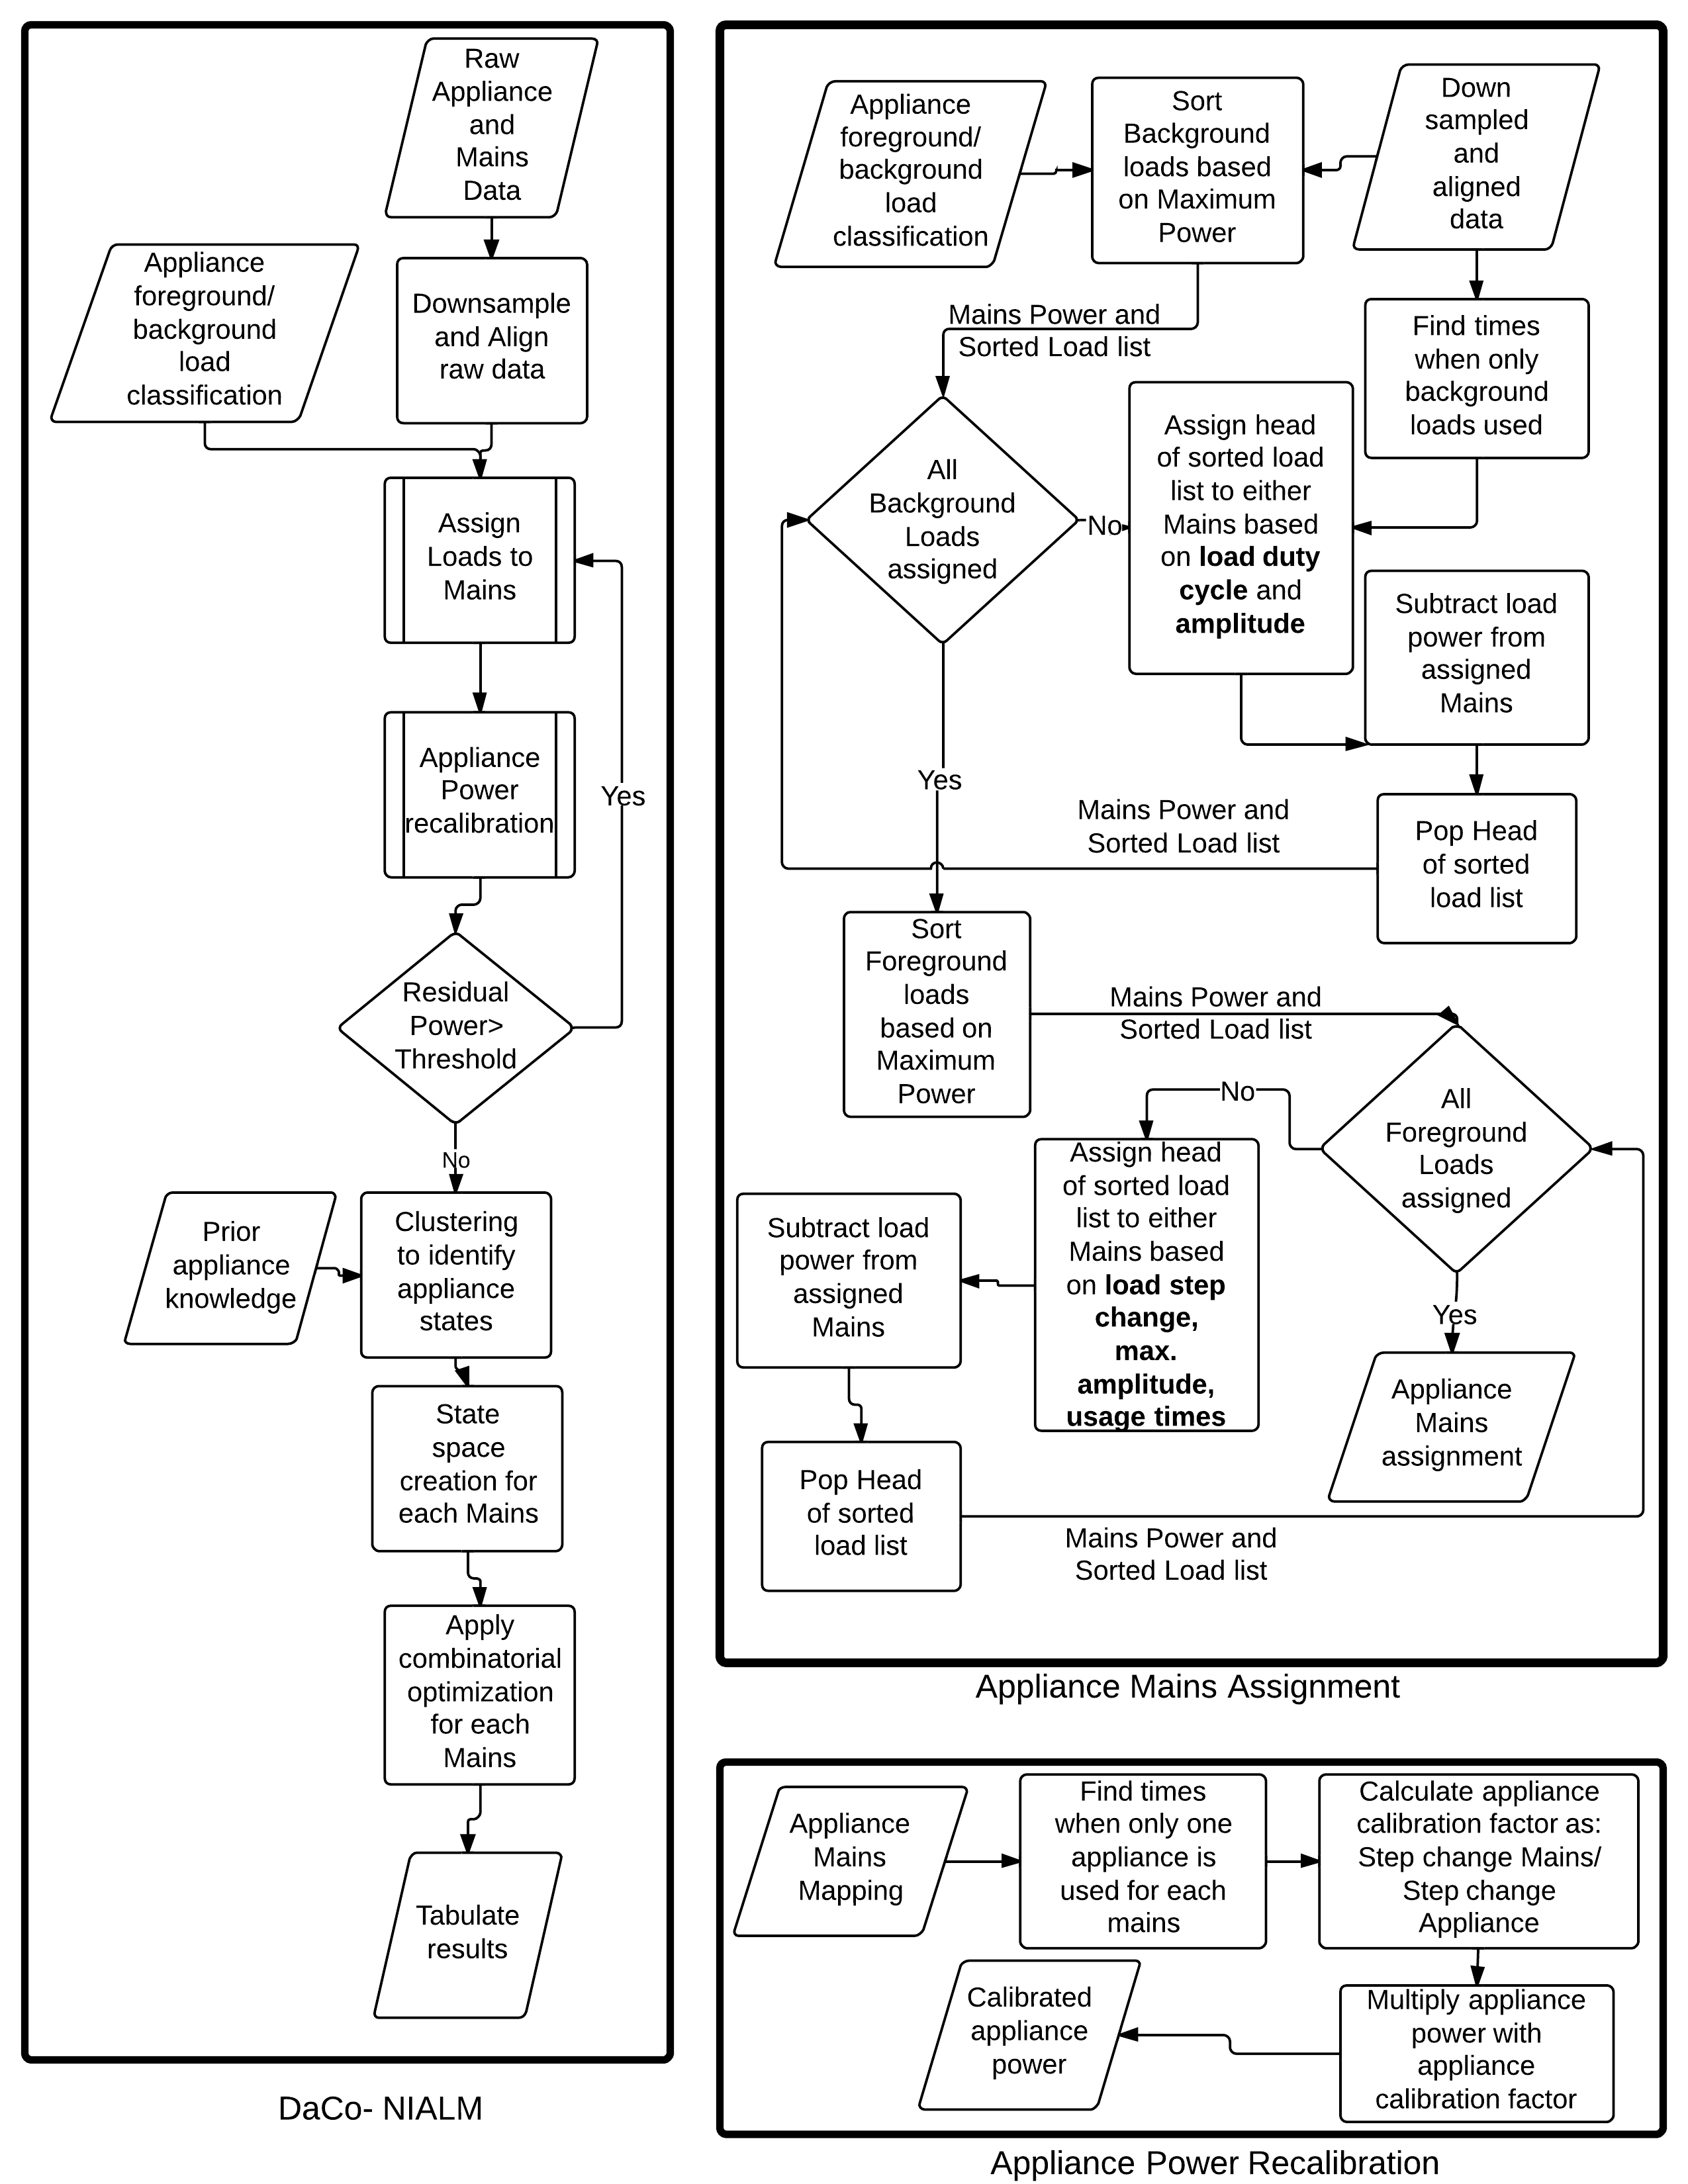
\includegraphics[scale=0.1]{./figures/algo_3.png}
%\caption{Divide and Conquer NIALM}
%   \label{fig:algorithm}
%\end{figure}
\noindent In this section we explain our algorithm- Improved Non intrusive load monitoring using load Division and Calibration (\indic). \indic provides preprocessing procedures which can simplify NIALM. These procedures can broadly be classified as data cleaning (time series synchronization, downsampling and calibration) and problem division into subproblems (assigning loads to mains). \indic can be used with any modeling technique described in Section II. Here, we present INDiC-CO (INDiC using Combinatorial optimization as modeling approach). CO proposed by Hart\cite{hart} is the simplest NIALM approach and by preprocessing using \indic  its shortcomings can be overcome. The various steps of INDiC-CO NIALM shown in \algoref{algo:main} are described below. 

\noindent\textbf{Time series synchronization}: Mains power and appliance power data are measured using different hardware\footnote{In REDD\cite{redd} TED meters(http://goo.gl/CEu2y) are used to measure mains and Power House Dynamics(http://goo.gl/9VQba) to measure appliance circuits}. It is highly likely that some hardware malfunctions during the data collection process. In this step we ensure that the mains power and appliance power time series start and end at the same time. Further missing data is handled using techniques such as forward filling (padding)\footnote{http://goo.gl/FfR6o}.

\noindent\textbf{Downsampling}: While performing CO it is desired that transients and fluctuations in the power signal are filtered\cite{hart}. The transients occur due to the high starting current of the appliance, whereas the fluctuations are a consequence of minor voltage fluctuations and oscillatory nature of appliances. \figref{fig:downsample_startup} and \figref{fig:downsample_voltage} show how starting current and voltage fluctuations can be filtered by down sampling. Filters such as mean/median can be used to down sample a time series to a time window, where the value assigned to a time window is the mean/median of values occurring during that time window in the original series.
%To overcome these we downsampled our data to one minute resolution using mean filter. 

\begin{figure} 
	
    \subfloat[\scriptsize When the compressor of refrigerator is turned on it consumes a very high starting power for a few seconds. This figure shows how these starting peak power can be filtered by downsampling to a suitable resolution]{
    \label{fig:downsample_startup}
    
    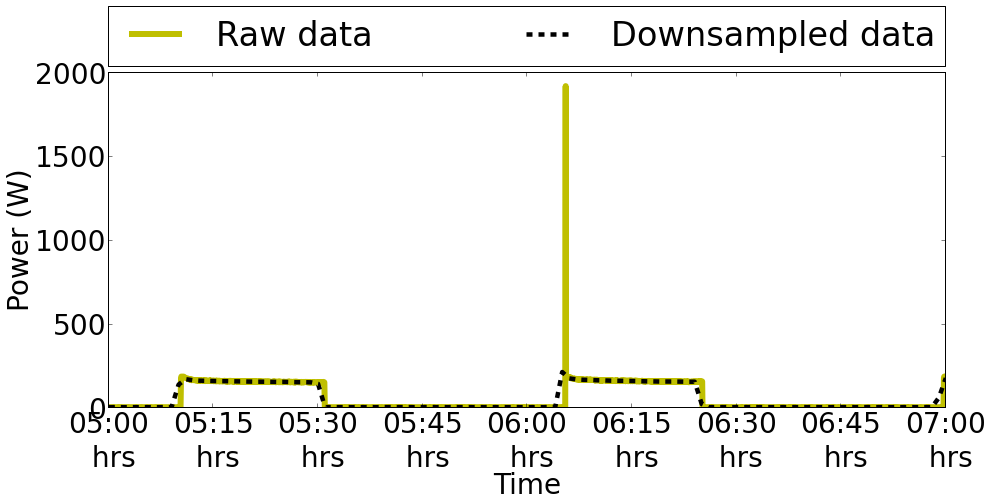
\includegraphics[scale=0.11]{./figures/downsample_1.png}}
    \hspace{1pt}
    \subfloat[\scriptsize Due to voltage fluctuations and oscillations the power consumed by an appliance can vary. This figure shows how these fluctuations can be reduced by downsampling to a suitable resolution]{
        \label{fig:downsample_voltage}
        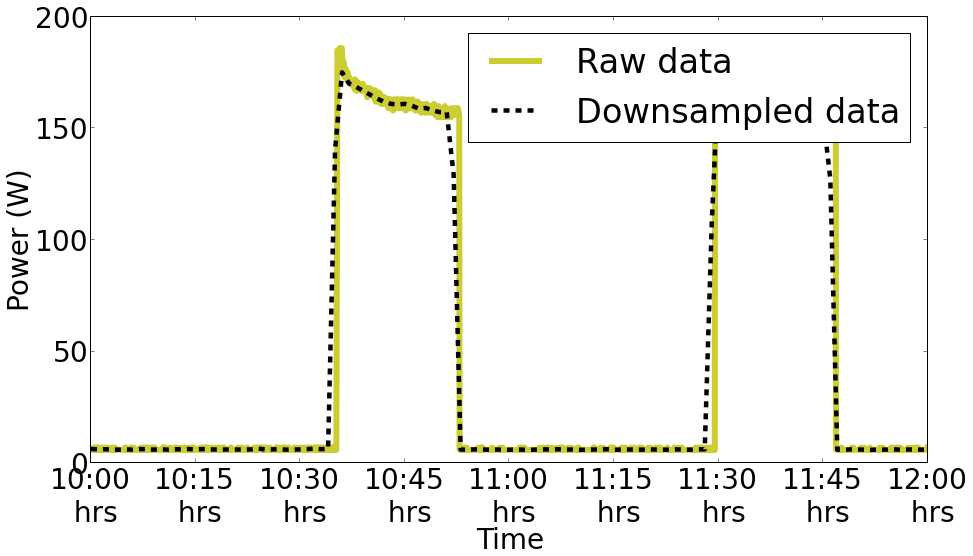
\includegraphics[scale=0.11]{./figures/downsample_2.png}}
    \vspace{-8pt}
  	\caption{Effect of downsampling appliance data}
  	\vspace{-20pt}
    \label{fig:downsampling}
\end{figure}

\noindent\textbf{Assigning Loads to Mains\footnote{While our approach is fine tuned for 2 Mains it can be easily extended to support further load division}}:
This step aims to identify the mapping ($Mapping[n]$) between appliances and mains. Since an appliance can belong to a single mains, $Mapping[n]$ is a one-to-one function from an appliance $n$ to a mains. Patterns corresponding to appliances having higher peak power are generally easier to extract from main signal, thus we sort the appliance in decreasing order of peak power. Starting from the appliance having highest peak load we compare its power at all times with the power of a mains. If at any time the power of the appliance is greater than the power of a mains, we can assign the appliance to the other mains. However, if we are not able to assign an appliance to mains this way, we find the times when $Events$ occur in the appliance power series. This should be a subset of times of $Events$ occurring in one of the mains to which this appliance is assigned. The threshold used to find events should be suitably chosen to ensure that minor voltage fluctuations are not counted as events. After an appliance has been assigned to a mains, its power sequence is subtracted from the corresponding mains to simplify mains assignment for remaining appliances. \figref{fig:assignment_1} shows how refrigerator is assigned to mains 2 since during this time interval its power is more than that of mains 1. Also, one may verify it by observing that the events in mains 2 and refrigerator power series occur at same time.
\begin{figure} 
	
    \subfloat[\scriptsize Assigning refrigerator to Mains 2 since refrigerator power $>$ Mains 1 power and events in Mains 2 and refrigerator occur at same time]{
    \label{fig:assignment_1}
    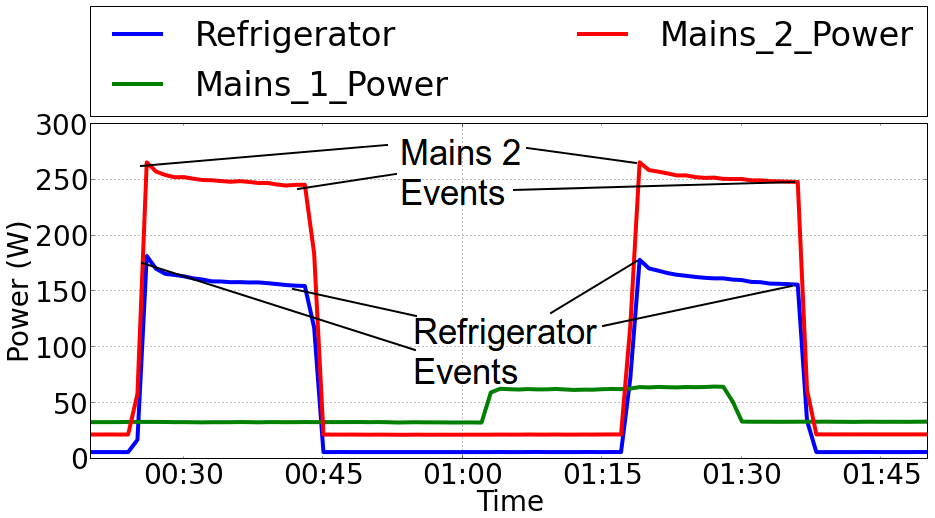
\includegraphics[scale=0.125]{./figures/calib.png}}
     \hspace{2pt}
    \subfloat[\scriptsize It can be seen that the magntude of event in mains 2 is significantly more than that in refrigerator. The ratio of these magntiudes is multiplied to refrigerator's power in this state (shown by black dotted line) to obtain calibrated power in this state (shown by yellow dotted line)]{
        \label{fig:assignment_2}
       
        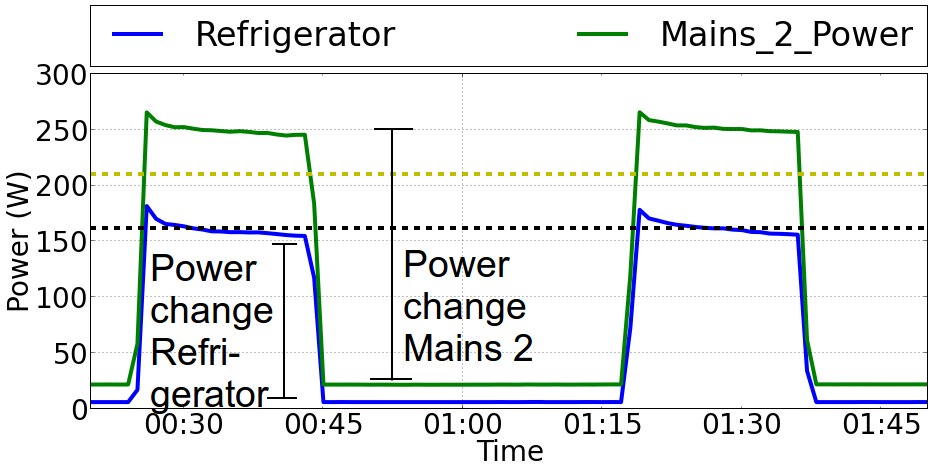
\includegraphics[scale=0.125]{./figures/calib_4.png}}
    \vspace{-8pt}
  	\caption{Calibrating and assigning refrigerator to Mains 2 }
  	\vspace{-20pt}
    \label{fig:assignment}
\end{figure}

\noindent\textbf{Clustering}: Prior knowledge and appliance circuitry\cite{ting2005} are used to identify the number of states associated with an appliance. For instance, a refrigerator is a compressor based appliance and exhibits three states in increasing order of power demand (compressor Off, compressor On, defrost mode). We use state of the art clustering techniques to cluster appliances' power draw using prior knowledge about number of appliance states.

\noindent\textbf{Appliance Power Calibration}: 
Power measured by appliance level meters may need calibration due to the following reasons:
\begin{itemize}
\item Different hardware report different measurement for same appliance \cite{berges2008}
\item Fluctuation in voltage causes power to fluctuate as well\cite{hart}
\item Missing meta data, whether real or apparent power is being measured at appliance level

\end{itemize} In comparison to appliance data, mains data is usually measured using better precision hardware. Thus, we keep mains data as a reference and calibrate appliance data against it. In the clustering step, value of appliance power at each time is associated with corresponding cluster state ($k \in {1,K}$). Since in Off state ($k$=1) appliance power consumption is almost zero, it does not require any calibration. We find out $Event$ times when appliance transitions from a lower state($k$) to a higher state($k+1$). During these times, we find the ratio of the magnitude of power change occurring in the assigned mains and the appliance. This ratio serves as a corrective multiplicative factor for a particular  state of an appliance. Cluster centroids obtained in the previous step are multiplied by this factor to obtain calibrated cluster centroids.
This process is shown in \figref{fig:assignment_2} where it is found that before calibration refrigerator power in state 2 was 162 W, after calibration with mains 2, it is found to be 210 W, where the calibration factor was found to be 1.3)

\noindent\textbf{Combinatorial optimization}: Combinatorial optimization is now performed separately for both mains as per the description in Section III.




\begin{algorithm}[ht!]
\DontPrintSemicolon % Some LaTeX compilers require you to use \dontprintsemicolon instead 
\KwIn{$x,\theta^n,\theta^{M_1},\theta^{M_2}$	}
\KwOut{$y^n,\mu_k^n$}
\BlankLine
\textbf{Time series synchronization}\;
\BlankLine
\nl$\theta^1,..\theta^n,\theta^{M_1},\theta^{M_2} \gets Timeseries\_sync([\theta^1,..\theta^n,\theta^{M_1},\theta^{M_2}],forward\: fill)$\;
\BlankLine
\textbf{Downsampling}
\BlankLine
\nl \For {$n \in {1,N}$}
	{
	$\theta^n \gets Downsample(\theta^n,mean,resolution)$\;
	}
\nl $\theta^{M_1} \gets Downsample(\theta^{M_1},mean,resolution)$\;
\nl $\theta^{M_2} \gets Downsample(\theta^{M_2},mean,resolution)$\;


\nl $j \gets Sort([\theta^1,..\theta^n],peak\: power)$\;
\BlankLine
\textbf{Appliance to Mains mapping}\;
\BlankLine
\nl \For{$Appliance\: n \in j$}
	{
	
\nl	\If {$\theta^n_t > \theta^{M_1}_t\: for\: any\: t \in {1,T}$} 
		{ $Mapping[n]=M_2$\;		
		}  
\nl	\ElseIf {$\theta^n_t > \theta^{M_2}_t\: for\: any\: t \in {1,T}$}
		{ $Mapping[n]=M_1$\;
		}
%\nl	\ElseIf {$n \in B$}
%		{
%\nl		$w \gets Contiguous\_Below\_Mean (\theta^{M_1}, 2\: hours)$\;
%		}
%\nl	\ElseIf {$n \in F$}
%		{
%		$w \gets Greater\_Than(\theta^n,100)$
%		}
\nl	\Else{
\nl		\If {$Event\_Detection(\theta^n,threshold).Times \subset Event\_Detection(\theta^{M_1},threshold).Times$ %\linebreak \&\: 
%		Step\_Changes(\theta^n,15,w).Magnitude \div \linebreak
%		Step\_Changes(\theta^{M_1},15,w).Magnitude \approx Constant\:C$
		}
			{ 
			$Mapping[n]=M_1$\;
			}
\nl		\Else{
			$Mapping[n]=M_2$\;	
			}	
		}
	\nl	$\theta^{Mapping[n]} \gets \theta^{Mapping[n]} - \theta^n $ \;
	}
	\BlankLine
	\textbf{Divide data into train and test set}\;
	\BlankLine
	
		
		\BlankLine
		\textbf{Clustering on train set}\;
		\BlankLine
	\nl	\For{$n \in {1,N}$}{
	\nl	$\mu_k^n \gets Cluster(\theta^n,K,clustering\_algorithm) \: for\: k \in {1,K} $\;
	}
	\BlankLine
	\textbf{Calibration on train set} \;
	\BlankLine
\nl	\For{$n \in {1,N}$}{    
\nl	\For{$k \in {2,K}$}{
	\nl	$\mu_k^n \gets \frac{\mu_k^n *Event\_Detection(\theta^{Mapping[n]}_{k-1,k},threshold).Magnitude}
				{ Event\_Detection(\theta^n_{k-1,k},threshold).Magnitude} $ \;
	}
%	
%\nl	$\theta^n \gets \frac{\theta^n * Step\_Changes(\theta^n,15,w).Magnitude}
%			{Step\_Changes(\theta^{M_{Mapping[n]}},15,w).Magnitude} $ \;
%\nl	$\theta^n \gets Normalize(\theta^n,v)$\; 
	
}


\BlankLine
\textbf{Combinatorial optimization on test set} \;
\BlankLine	
	
\nl Solve combinatorial optimization as described in Section III

\nl \Return{$y^n,\mu_k^n$}\;
\caption{INDiC-CO}
\label{algo:main}

\end{algorithm}


\section{Evaluation}

\noindent We use Reference Energy Disaggregation Data Set (REDD) \cite{redd} for validating our algorithms based on metrics such as Mean normalized error (MNE) and RMS error (RE) proposed in previous work.
\subsection{About dataset}
\noindent REDD contains power data for mains (2 phases) as well as appliances from 6 homes in Boston area collected in the summer of 2011. The data is made available as raw, high frequency (sampled at 15 KHz) and low frequency (Mains at 1 Hz, appliances at ~0.3 Hz). Considering the practical implications of residential smart meter installation, we believe that low frequency data represents the most realistic scenario and thus we use this data for analysis. 

%\figref{fig:breakdown} shows 6 hourly breakdown of energy consumption across the different mains in Home 2 .


%\begin{figure} 
%	
%    \subfloat[\scriptsize Mains 1]{
%    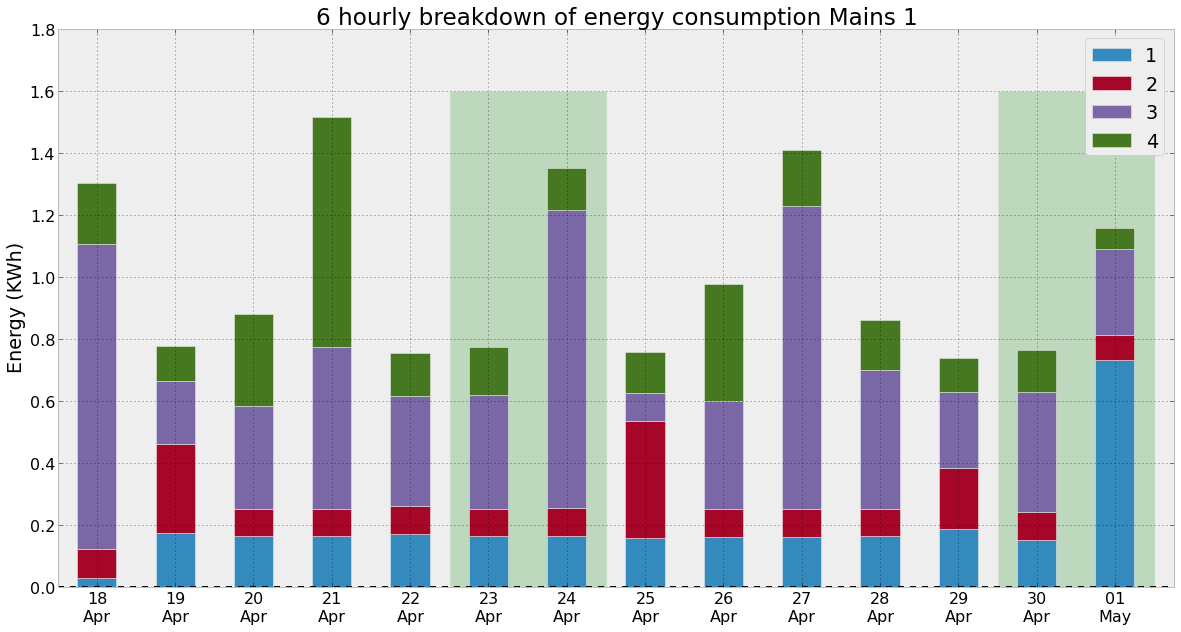
\includegraphics[scale=0.1]{./figures/mains_1_6hr.png}}
%    \subfloat[\scriptsize Mains 2]{
%        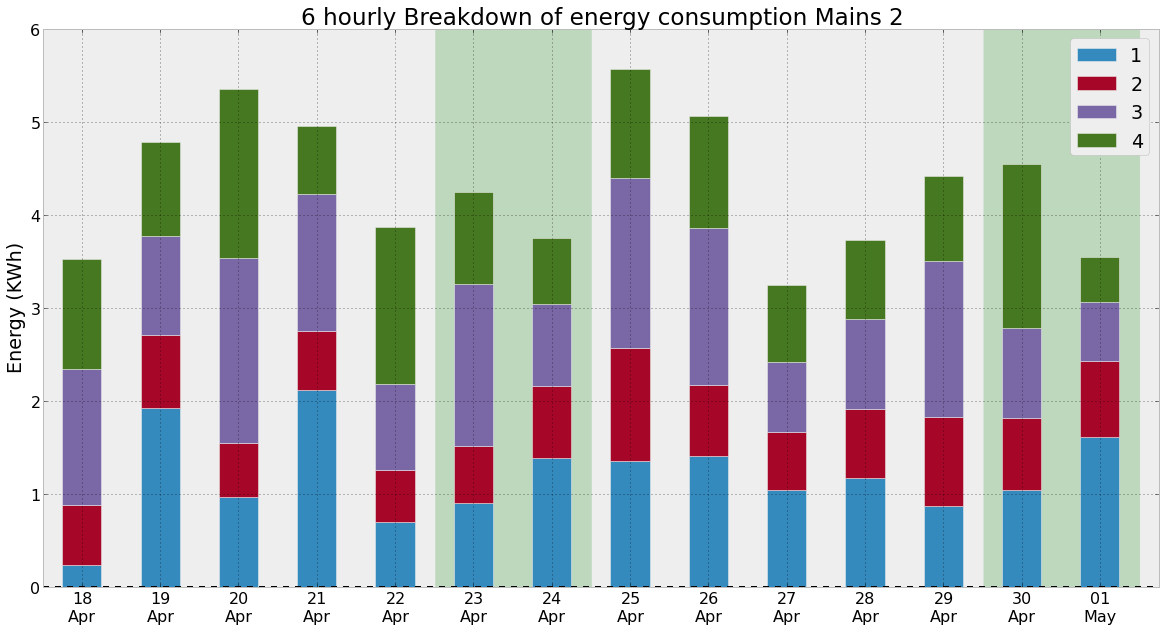
\includegraphics[scale=0.1]{./figures/mains_2_6hr.png}}
%  	\caption{6 hourly energy usage breakdown Home 2}
%    \label{fig:breakdown}
%\end{figure}
%
\subsection{Evaluation Metric}

\noindent Commonly used metrics such as accuracy, sensitivity and specificity can be misleading when applied to NIALM. We illustrate this with the help of a confusion matrix whose [m,n] entry in indicates the number of times appliance in state $m$ is predicted to be in state $n$. It can be seen from the confusion matrix in \figref{fig:confusion} that since stove is mostly in state 1 (Off), accuracy will be largely decided by accuracy for this state. This will overshadow the accuracy for state 2 (On) which is unintended.
%Armel et. al \cite{survey1} discuss the lack of a common metric while comparing NIALM approaches.
Thus, we use the following metrics which have been used in the past work \cite{parson2012_aaai,redd}:

\noindent\textbf{Mean Normalized Error (MNE\%)}: Normalized error in the energy assigned to an appliance $n$ over time period $T$, given by:
\begin{equation}
MNE(n)=\frac{|\sum\limits_{t=1}^{T}\theta_t^n-\sum\limits_{t=1}^{T}y_t^n|}{\sum\limits_{t=1}^{T}\theta_t^n} 
\end{equation} 

\noindent The above metric will give a 0\% MNE for cases such as follows: $y^n=[0,10,0,10]$ and $\theta^n=[10,0,10,0]$, which can be misleading. Thus, we propose a modified Mean Normalized Error metric further referred as MNE which is sensitive to such cases.
\begin{equation}
MNE(n)=\frac{\sum\limits_{t=1}^{T}|\theta_t^n-y_t^n|}{\sum\limits_{t=1}^{T}\theta_t^n} 
\end{equation} 
\noindent Since it is a known fact that $|\sum a-\sum b| \le \sum|a-b|$ where $a$ and $b$ are vectors containing floating point numbers, our results might look worse than if the original definition of MNE were used.

\noindent\textbf{RMS Error (RE Watts)}: RMS error in power assignment to an appliance $n$ per time slice $t$ given by:
\begin{equation}
RE(n)=\sqrt{\frac{1}{T}\sum\limits_{t=1}^{T}(\theta_t^n-y_t^n)^2}
\end{equation}


\noindent Both these quantities represent error, the lesser they are the better is the prediction.
%\begin{table}
%\begin{tabular}{content...}
%content...
%\end{tabular}
%\end{table}

%\begin{figure}
%\centering 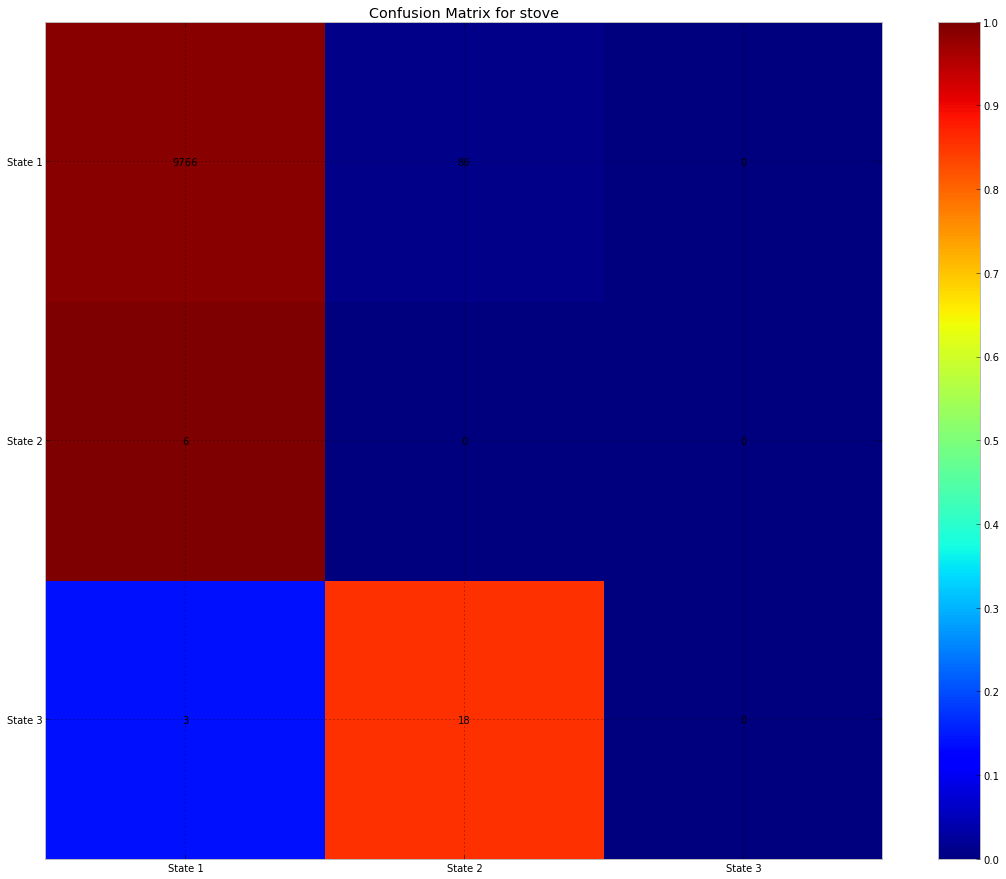
\includegraphics[scale=0.15]{./figures/confusion_stove.png}
%\vspace{-8pt}
%\caption{Confusion Matrix showing predicted state accuracy for Stove}
%   \label{fig:confusion}
%   \vspace{-20pt}
%\end{figure}



\subsection{Empirical Analysis}
\noindent We performed empirical analysis on REDD dataset Home 2, which consists of 11 channels (including 2 mains and 9 appliances)\footnote{Highest accuracy has been reported for this Home in previous work\cite{redd}}. We believe that the same analysis can be easily repeated across multiple homes. Timeseries synchronization was applied since the appliance level data collection begun about 6 hours after mains data collection. Moreover, there were small intervals of missing data, which we filled using forward filling. Two appliances - washer dryer and disposal were ignored from further analysis since washer dryer had a peak power consumption of 8 W (which means it was Off throughout) and the contribution of disposal to overall power was less than 0.1 \%.  We downsampled this time synchronized data to one minute resolution using mean filter. 1 minute is a sufficient resolution to get rid of startup transients and voltage fluctuations. As per the Appliance to Mains step in INDiC-CO algorithm described earlier we assigned loads to the two different mains.  \tabref{tab:calibration_factors} shows the assignment of loads to different mains. Further this table also shows the learnt power states of these appliance via KMeans++\footnote{We used DBScan, SOM, EM and Hierarchial clustering apart from KMeans++, but found KMeans++ to be most scalable} \cite{kmeansplusplus} clustering. Refrigerator and lighting showed significant difference in power states post calibration. Based on prior experience and appliance circuity\cite{ting2005}, we believe that since only these two appliances needed calibration, it may be a case that the appliance level monitor measured real power instead of apparent power. These two loads constitute a major chunk of mains 2 power. \figref{fig:calibration} shows the reduction in unassigned power due to calibrating these two appliances. 

\noindent To show the significance of load division and calibration as a preprocessing step to NIALM algorithm, we considered 4 possible cases:  i) no calibration, no load division; ii) no calibration, load division; iii) calibration, no load division; iv) calibration, load division (INDiC). The results after applying INDIC-CO are presented in \tabref{tab:results}. For the overall dataset, it can be seen that MNE reduces from 187\% to 39\%, RE reduces from 478 W to 168 W, after applying INDiC-CO. All appliances show reduction in MNE and RE after applying INDiC-CO. However, there is significant improvement in correctly predicting refrigerator and lighting. \figref{fig:confusion_ref} shows the confusion matrix for refrigerator prediction pre and post applying INDiC-CO. It can be seen that after applying INDiC there is a vast improvement in predicting refrigerator's state 1 and 2.
%
%\noindent We had used Combinatorial Optimization which is the simplest NIALM technique to show the improvements which can be made by load division and appliance calibration. We believe that using state of the art NIALM algorithms will improve the results by leaps and bounds.

%\item Overall results in \tabref{tab:results}, first column NILM without dividing into mains and without recalibration, last column with DiCaCo NIALM. Vast reduction in R.E. and M.N.E , especially for most appliance contributing most like refrigerator and lighting	
%\item Confusion matrix showing a large improvement in refrigerator recognition in \figref{fig:confusion_ref}
%\end{itemize}

\begin{figure} 
	
    \subfloat[\scriptsize Without applying calibration, more than one-thirds of total power in mains 2 is unaccounted. This can significantly reduce accuracy when any NIALM model is applied]{
    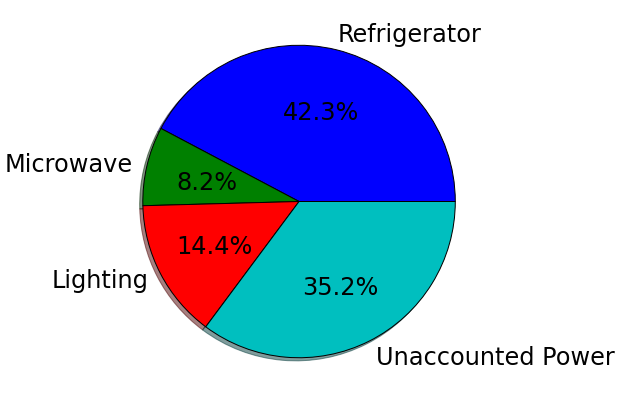
\includegraphics[scale=0.2]{./figures/breakdown_before_calibration.png}}
    \hspace{1pt}
    \subfloat[\scriptsize After applying calibration, unaccounted power reduces to less than 10\% of mains 2 power. The contribution of refrigerator and lighting to overall mains 2 power increaes. ]{
        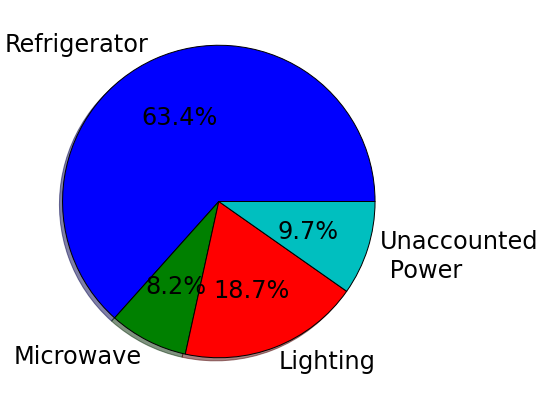
\includegraphics[scale=0.2]{./figures/breakdown_after_calibration.png}}
  	\caption{Mains 2 Break down by load}
  	\vspace{-8pt}
    \label{fig:calibration}
    \vspace{-20pt}
\end{figure}


% % % % % % Confusion Matrix Result Images % % % % % % % % % % % % % %

\begin{figure} 
	
    \subfloat[\scriptsize Confusion matrix for refrigerator after applying CO based NIALM. State 2 is predicted to be in state 3 more than in state 2]{
    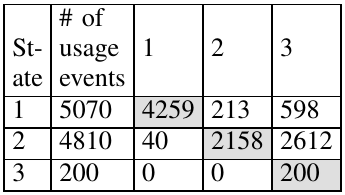
\includegraphics[scale=0.355]{./figures/confusion_before_big.png}}
    \hspace{2pt}
    \subfloat[\scriptsize Confusion matrix for refrigerator after applying INDiC-CO based NIALM. There are more instances along the diogonal sginfifying improvement in prediction. State 2 shows significant improvements.]{
        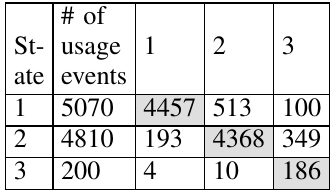
\includegraphics[scale=0.355]{./figures/confusion_after_big.png}}
        \vspace{-8pt}
  	\caption{Confusion Matrices for refrigerator disaggregation. [m,n] in the matrix represents appliance's $m^{th}$ state to be predicted as $n^{th}$ state. Grey cells along the diagonal show true positive.}
  	
    \label{fig:confusion_ref}
    \vspace{-20pt}
\end{figure}


% % % % % Confusion Matrix results in table % % % % % % % % % % % % % % % % % % % % % % % % % %
%\begin{table}[!htb]
%    \caption{Confusion Matrices for NIALM. [m,n] in the matrix represents appliance's $m^{th}$ state to be predicted as $n^{th}$ state. Grey cells along the diagonal show true positive.}
%%    \begin{minipage}{.28\linewidth}
%%      \caption{}
%%      \centering
%%      \tabcolsep=0.07cm
%%        \begin{tabular}{|l|l|l|l|}
%%        \hline
%%                  & \# of &  &\\
%%             St-& usage& 1 & 2\\
%%             ate     & events&&\\
%%         \hline
%%         1&10049&\cellcolor{gray!25}9616&443\\
%%         \hline
%%         2&21&11&\cellcolor{gray!25}10\\
%%         \hline
%%        \end{tabular}
%%    \end{minipage}%    
%           \begin{minipage}{.45\linewidth}
%           \centering
%             \caption{Confusion matrix for refrigerator after applying CO based NIALM. State 2 is predicted to be in state 3 more than in state 2}
%             \tabcolsep=0.07cm
%             \begin{tabular}{|l|l|l|l|l|}
%                     \hline
%                               & \# of &  &&\\
%                          St-& usage& 1 & 2& 3\\
%                          ate     & events&&&\\
%                      \hline
%                      1&5070&\cellcolor{gray!25}4259&213&598\\
%                      \hline
%                      2&4810&40&\cellcolor{gray!25}2158&2612\\
%                      \hline
%                      3&200&0&0&\cellcolor{gray!25}200\\
%                      \hline
%                 \end{tabular}
%             \end{minipage}
%             \begin{minipage}{.45\linewidth}
%                            \centering
%                              \caption{}
%                              \tabcolsep=0.07cm
%                              \begin{tabular}{|l|l|l|l|l|}
%                                      \hline
%                                                & \# of &  &&\\
%                                           St-& usage& 1 & 2& 3\\
%                                           ate     & events&&&\\
%                                       \hline
%                                       1&5070&\cellcolor{gray!25}4457&513&100\\
%                                       \hline
%                                       2&4810&193&\cellcolor{gray!25}4368&349\\
%                                       \hline
%                                       3&200&4&10&\cellcolor{gray!25}186\\
%                                       \hline
%                                  \end{tabular}
%                              \end{minipage}  
%\end{table}

%\item Table on Calibration factors
\begin{table}
%%% increase table row spacing, adjust to taste
%%\renewcommand{\arraystretch}{1.3}
%% if using array.sty, it might be a good idea to tweak the value of
%% \extrarowheight as needed to properly center the text within the cells
\caption{Mains assignment and appliance states power. Lighting and refrigerator power shows change after calibration}
\vspace{-8pt}
\label{tab:calibration_factors}
%\centering
%%% Some packages, such as MDW tools, offer better commands for making tables
%%% than the plain LaTeX2e tabular which is used here.
\begin{tabular}{|c|c|c|c|c|c|c|c|}
\hline
Appliance & Mains & \multicolumn{6}{|c|}{States Power (W)}\\
\hline
&&\multicolumn{3}{|c|}{Pre calibration}&\multicolumn{3}{|c|}{Post calibration}\\
\hline
Refrigerator & 2& 7&162&423 & 9&210&423\footnote{Could not be calibrated}\\
Microwave &2& 10&832&1730& 10&832&1730\\
Lighting & 2& 9&96&156&10&110&178\\
Dishwasher & 1& 0&256& 1195 & 0&256& 1195\\
Stove& 1 & 0&374&-& 0&374&-\\
Kitchen & 1& 5&727&-&5&727&-\\
Kitchen 2&1 & 1&204&1032&1&204&1032 \\
%
%
\hline
%
\end{tabular}
\end{table}

\begin{table}
\caption{MNE and RE for CO based NIALM with and without INDiC. Results for INDiC-CO are highlighted in grey}
\vspace{-8pt}
\label{tab:results}
\begin{tabular}{|p{30pt}|p{12pt}|p{14pt}|p{12pt}|p{14pt}|p{12pt}|p{14pt}|a|a|}
\hline
&\multicolumn{4}{|c|}{Without}&\multicolumn{4}{|c|}{With}\\
&\multicolumn{4}{|c|}{calibration}&\multicolumn{4}{|c|}{calibration}\\
\hline
&\multicolumn{2}{|c|}{Without load}&\multicolumn{2}{|c|}{With load}&\multicolumn{2}{|c|}{Without load}&\multicolumn{2}{|c|}{With load}\\
&\multicolumn{2}{|c|}{division}&\multicolumn{2}{|c|}{division}&\multicolumn{2}{|c|}{division}&\multicolumn{2}{|c|}{division}\\
\hline

Appliance &R.E.&M.N.E.& R.E.&M.N.E.&R.E.&M.N.E.&R.E.& M.N.E.\\
&Watts&\%&Watts&\%&Watts&\%&Watts&\%\\
\hline
Refrigerator & 136 &109 & 71 & 32 & 130 &95  &59 &21\\
Microwave    & 102 &98  & 97 & 110& 104 &97  &96 &109\\
Lighting     & 51  &164 & 48 & 195& 44  &83  &38 &60\\
Dishwasher   & 406 &2947& 63 & 100& 377 &2517&63 &100\\
Stove        & 77  &1191& 36 & 281& 75  &1118&36 &281\\
Kitchen      & 64  &182 & 58 & 168& 69  &196 &58 &168\\
Kitchen 2    & 95  &267 & 91 & 117& 92  &230 &91 &117\\
\hline
Overall      &478  &187 &161 &  58& 450 &157 &168&39\\

\hline

\end{tabular}
\end{table}





\section{Conclusion and Future Work}
\noindent In this paper we present \indic which consists of preprocessing steps which can reduce the complexity of following NIALM model. We empirically show the improvements in disaggregation when simple and elegant preprocessing such as \indic are used. In the future we intend to apply \indic as a preprocessing step to other NIALM approaches. We plan to look into additional features such as correlation between multiple appliance usage, taking time of day into account. We also intend to apply \indic on other datasets, especially the ones from developing countries where loads are significantly different from the ones used in developed countries.

%\begin{itemize}
%
%\item Applying model on noisy datasets
%\item 2 D CO (when Real and Reactive Power are known)
%\item Factoring in Time of Day etc.
%\item Factoring in Appliance Correlation
%\item Factor in switch continuity, essentially leads to Factorial HMM
%\item Distributed NILM
%\item Adaptive Learning
%\end{itemize}
%
%\section*{Acknowledgment}
%The authors would like to thank TCS Research and Development for supporting the first author through PhD. fellowship. We would also like to thank NSF- DEITy for funding the project.
\bibliographystyle{IEEEtran}
\bibliography{IEEEabrv,references}

\end{document}


